Bevor eine künstliche Intelligenz einen E-Commerce Bereich optimieren kann, müssen ausreichend Daten bereit stehen und eine Systemanpassung für die KI erfolgen.

\subsection{Data Mining}
Um die künstliche Intelligenz zu trainieren können sollten folgenden Daten verwendet werden,

\begin{itemize}
	\item historische Verkaufsdaten
	\item Tracking Daten und Nutzerverhalten auf der Webseite, Aktionen und Interaktionen erfassen
	\item Adressdaten (soziale Brennpunkte, gut konstituierte Gegenden)
	\item Kundenstammdaten (Name, Geschlecht, Alter oder Unternehmensname)
	\item Kundenmeinungen und -bewertungen
	\item bevorzugte Produkte des Nutzers
	\item Warenkorbwert (geringer Warenkorbwerte bekommen keine Werbekampagnen, hohe erhalten sogar Premium Behandlung)
	\item saisonale Preisentwicklungen bei Produkten (z.B. Tannenbäume vor Weihnachten)
	\item geografische Lage
	\item aktuelle Trends
\end{itemize}

Sind die Daten erhoben müssen diese aufbereitet und selektiert werden, je nach Verwendungszweck der Daten. Nach \cite{laurenz_data_mining} lassen sich Data Mining Aufgaben in vier Gruppen unterteilen.\vspace{0.2cm}

\textit{Klassifizierung}: sucht anhand von Merkmalen nach Muster um Objekte zusammenzufassen. Im E-Commerce könnte das ein ,,gemeinsames Interesse an einem Produkt'' sein.\vspace{0.2cm}

\textit{Prognose}: erstellen anhand von Variablen Modelle zur Vorhersage einer abhängigen Variable. Dies kann zum Beispiel die ,,Umsatzentwicklung, anhand von Anzahl Bestellungen, Höhe des Warenkorbwertes'' prognostizieren.\vspace{0.2cm}

\textit{Segmentierung}: versucht mittels des Datenbestandes die Objekte in Segmente zufassen. Hier wird auch von ,,Cluster-Analyse'' gesprochen. Die Segmente sollen anhand von Merkmalen eines möglichst homogene Teilmenge ergeben.\vspace{0.2cm}

\textit{Assoziation}: mit ihrer Hilfe lassen sich Verbindungen zwischen verschiedenen Ziel – Variablen schaffen. Beispielsweise, ,,ein Kunde der Produkt A kaufte, dann kauft dieser auch, zu 80\% Produkt B''. Die Abbildung \ref{img:classification_data_mining_tasks} zeigt eine Zusammenfassung der Data Mining – Aufgaben.

\begin{figure}[!ht]
	\centering
	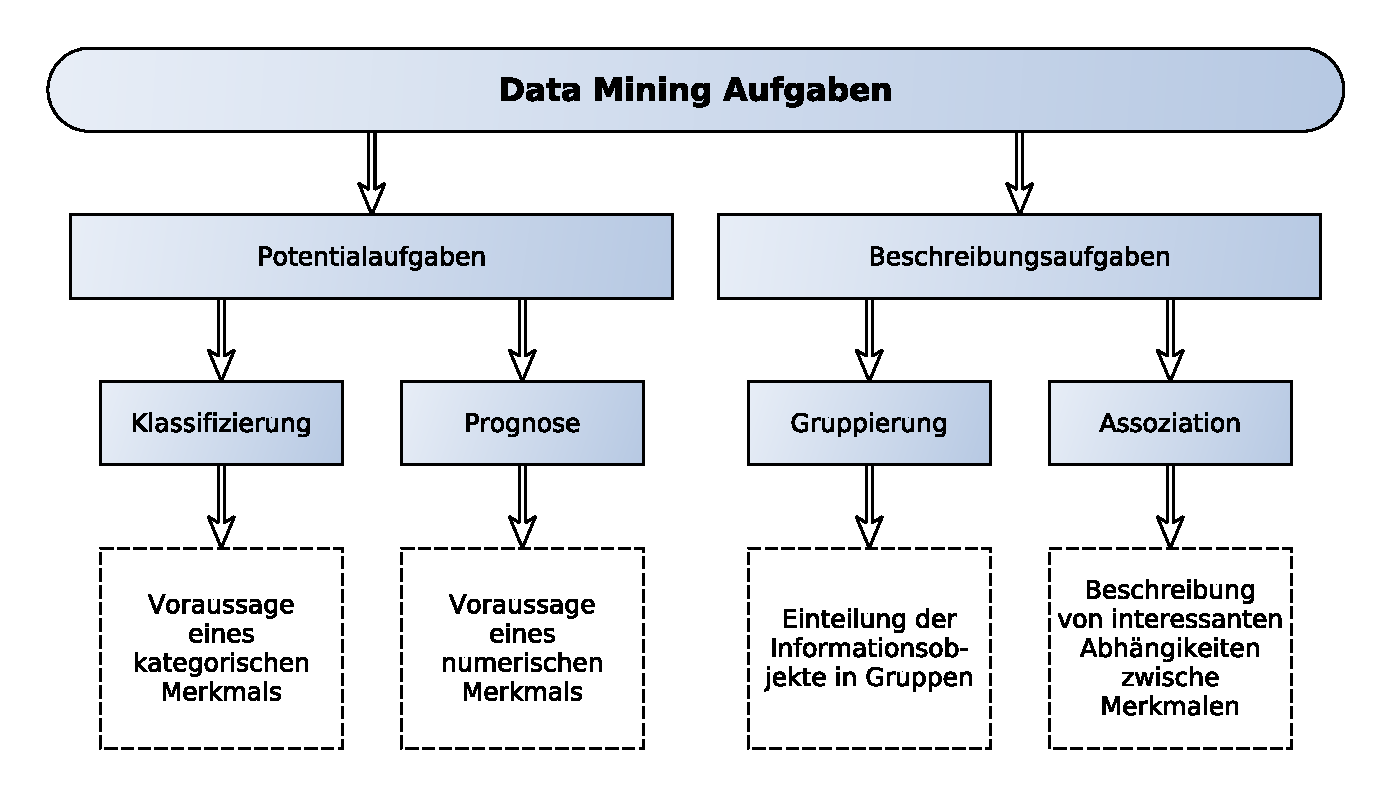
\includegraphics[width=\linewidth]{images/classification_data_mining_tasks.eps}
	\caption{Klassifizierung der Data Mining Aufgaben}
	\label{img:classification_data_mining_tasks}
\end{figure}

\subsection{Infrastruktur für künstliche Intelligenz im Onlinehandel}
Um dem Nutzer ein optimales Einkaufserlebnis zu ermöglichen, ist auch eine geeignete Infrastruktur erforderlich. Ein möglicher Ansatz ist in \cite{netz98_headless_commerce} und \cite{perske_headless_commerce} beschrieben. So können beispielsweise die Komponenten der künstlichen Intelligenz in einer Middleware, in der Abbildung \ref{img:infrastructor_for_ai_in_e__commerce} rot dargestellt integriert werden. Die Frontend-Anwendungen stellen eine Anfrage, zum Beispiel anzuzeigende ,,Produktempfehlungen'' und erhalten die passenden Daten von der Middleware, die die Datensysteme abfragt. Daten können dann simultan aus verschiedenen Systemen geholt, verarbeitet und direkt an die jeweiligen Frontend-Anwendungen gesendet werden. Die verschiedenen Frontend-Anwendungen und Services sind unabhängig von den Datensystemen umgesetzt und verwenden die Daten und Funktionen der Datensysteme. Die Frontend-Anwendungen sind der Abbildung \ref{img:infrastructor_for_ai_in_e__commerce} gelb dargestellt und die Systemen mit den Datenquellen und Funktionalitäten sind grün.

\begin{figure}[!ht]
	\centering
	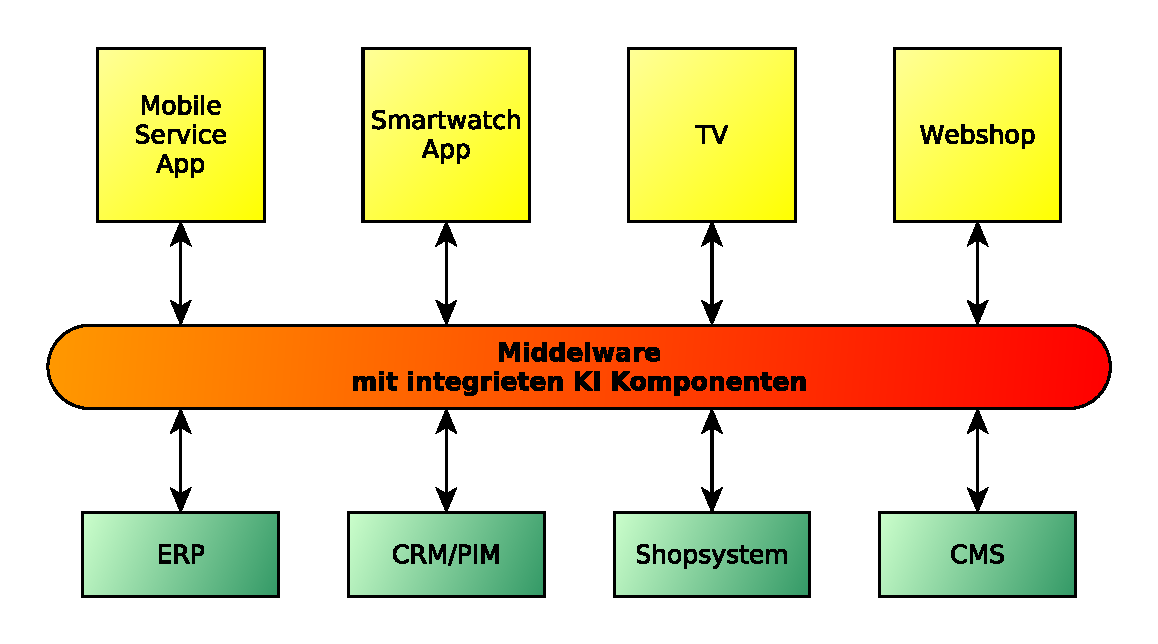
\includegraphics[width=\linewidth]{images/ecommerce-eco-system.eps}
	\caption{Mögliche Infrastruktur für künstlichen Intelligenz im Onlinehandel}
	\label{img:infrastructor_for_ai_in_e__commerce}
\end{figure}
